\begin{figure}[H]
\centering
\resizebox{0.45\textwidth}{!}
{
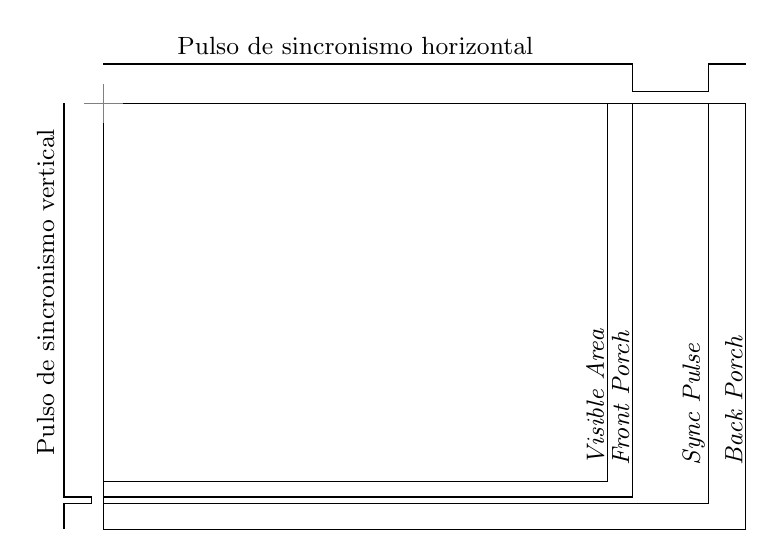
\begin{tikzpicture}[x = .1mm, y = .1mm]
    
    \def\hvisiblearea {640}
    \def\vvisiblearea {480}
    
    \def\hfrontporch {16 * 2} % alterado para ficar mais estetico
    \def\vfrontporch {10 * 2} %

    \def\hsyncpulse {96}
    \def\vsyncpulse {2 * 4} % alterado para ficar mais estetico

    \def\hbackporch {48}
    \def\vbackporch {33}

    \begin{scope}[xshift = 5mm, local bounding box = pulse horizontal]
        \draw [black] (0, 0) -- ++(\hvisiblearea + \hfrontporch, 0) -- ++(0, -3.5mm) -- ++(\hsyncpulse, 0) -- ++(0, 3.5mm) -- ++(\hbackporch, 0);
        \node [above, font = \small] at (\hvisiblearea / 2, 0) {Pulso de sincronismo horizontal};
    \end{scope}

    \begin{scope}[yshift = -5mm, local bounding box = pulse vertical]
        \draw [black] (0, 0) -- ++(0, -\vvisiblearea - \vfrontporch) -- ++(3.5mm, 0) -- ++(0, -\vsyncpulse) -- ++(-3.5mm, 0) -- ++(0, -\vbackporch);
        \node [above, font = \small, rotate = 90] at (0, -\vvisiblearea / 2) {Pulso de sincronismo vertical};
    \end{scope}
    
    \begin{scope}[xshift = 5mm, yshift = -5mm, local bounding box = screen]
        % visible area
        \draw [black] (0, -\vvisiblearea) -- ++(\hvisiblearea, 0) -- ++(0, \vvisiblearea);
        % front porch
        \draw [black] (0, -\vvisiblearea - \vfrontporch) -- ++(\hvisiblearea + \hfrontporch, 0) -- ++(0, \vvisiblearea + \vfrontporch);
        % sync pulse
        \draw [black] (0, -\vvisiblearea - \vfrontporch - \vsyncpulse) -- ++(\hvisiblearea + \hfrontporch + \hsyncpulse, 0) -- ++(0, \vvisiblearea + \vfrontporch + \vsyncpulse);
        % back porch
        \draw [black] (0, 0) rectangle ++ (\hbackporch + \hvisiblearea + \hfrontporch + \hsyncpulse, -\vbackporch - \vvisiblearea - \vfrontporch - \vsyncpulse);
    
        %
        \node[above right = 0.8mm, font = \small, rotate = 90] at (\hvisiblearea, -\vvisiblearea) {\textit{Visible Area}};
        \node[above right = 0.8mm, font = \small, rotate = 90] at (\hvisiblearea + \hfrontporch, -\vvisiblearea) {\textit{Front Porch}};
        \node[above right = 0.8mm, font = \small, rotate = 90] at (\hvisiblearea + \hfrontporch + \hsyncpulse, -\vvisiblearea) {\textit{Sync Pulse}};
        \node[above right = 0.8mm, font = \small, rotate = 90] at (\hvisiblearea + \hfrontporch + \hsyncpulse + \hbackporch, -\vvisiblearea) {\textit{Back Porch}};
    \end{scope}

    \draw [gray, fill opacity = 0.5] (5mm,   -7.5mm) -- ++(0,    5mm);
    \draw [gray, fill opacity = 0.5] (7.5mm, -5mm)   -- ++(-5mm, 0);
\end{tikzpicture}
}
\caption{Regiões de varredura da tela}
\end{figure}